\documentclass[10pt,a4paper]{article}
\usepackage[utf8x]{inputenc}
\usepackage{ucs}
\usepackage{amsmath}
\usepackage{amsfonts}
\usepackage{amssymb}
\usepackage{a4wide}
\usepackage{comment}
\usepackage[pdftex]{graphicx}
\usepackage{epstopdf}
\newcommand{\cmd}[1]{\texttt{#1}}
\newcommand{\remove}{}
\newcommand{\dir}[1]{\textsf{#1}}
\newcommand{\pop}{Depiler\xspace}
\newcommand{\push}{Empiler\xspace}
\newcommand{\tete}{LireTete}
\newcommand{\sommet}{LireSommet}
\newcommand{\empt}{EstVide}
\newcommand{\enqueue}{Enfiler\xspace}
\newcommand{\dequeue}{Defiler\xspace}
\newcommand{\get}{\ensuremath{\leftarrow\ }}

\usepackage[textsize=small, textwidth=2cm, color=yellow]{todonotes}

\excludecomment{solution}
\includecomment{solution}

\title{IF111 - Algorithmes et structures de données-TD4 :\\ Rappels}
\date{}
\author{\underline{Jonathan Narboni}, Rohan Fossé}
\date{\underline{\texttt{jonathan.narboni@labri.fr}}, \texttt{rfosse@labri.fr}}


\begin{document}
\maketitle

\section*{Exercice 1}
Étant donné un tableau trié de n entiers distincts où chaque entier est compris entre 0 et m-1 et m>n. Recherchez le plus petit nombre manquant dans le tableau. Proposez un algorithme avec une complexité logarithmique $\mathcal{O}(log(n))$.\\
Par exemple, si l'on considère le tableau [0, 1, 2, 6, 9] avec n = 5 et m = 10, alors l'algorithme donnera 3.

\section*{Exercice 2}
Écrire une fonction fusion qui prend en argument deux listes triées L1 et L2 et qui renvoie une seule liste triée contenant les éléments de L1 et L2.

\section*{Exercice 3}
 Le graphe ci-dessous représente le plan d'une ville.\\

Le sommet A désigne l'emplacement des services techniques.\\

Les sommets B, C, D, E, F et G désignent les emplacements de jardins publics. Une arête représente l'avenue reliant deux emplacements et est pondérée par le nombre de feux tricolores situés sur le trajet. \\

\begin{figure}[h!]
    \centering
    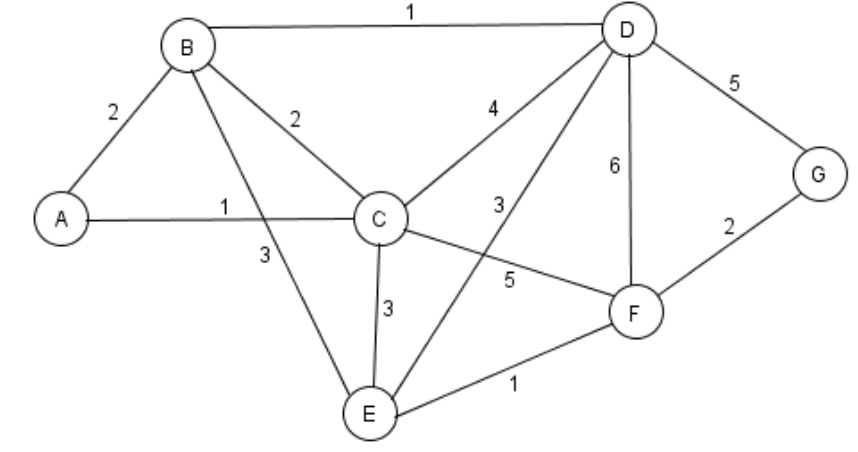
\includegraphics[scale=0.6]{Djisktra.png}
    \label{fig:my_label}
\end{figure}

 On s'intéresse au graphe non pondéré. Répondre aux questions suivantes :
\begin{enumerate}
    \item Ce graphe est-il connexe ?
    \item Ce graphe est-il complet ?
    \item Ce graphe admet-il une chaîne eulérienne ?
    \item Ce graphe admet-il un cycle eulérien ?
    \item Déterminer, en justifiant, le nombre chromatique de ce graphe.
\end{enumerate}
On s'intéresse dorénavant au graphe pondéré. Proposer un trajet comportant un minimum de feux tricolores reliant A à G.




\section*{Exercice 4}
Soit un groupe de personnes tel que :
\begin{enumerate}
    \item Chaque personne est membre d’exactement deux associations;
    \item Chaque association comprend exactement trois membres;
    \item Deux associations quelconques ont toujours exactement un membre en commun.
\end{enumerate}
Combien y a-t-il de personnes ? d’associations ?

\end{document}


